%/*******************************************************************************
% * Copyright (c) 2007, G. Weirich
% * All rights reserved. This program may not be distributed
% * or modified without prior written consent
% *
% * Contributors:
% *    G. Weirich - initial implementation
% *
% *  $Id: elexis-arzttarife-schweiz.tex 3941 2008-05-20 13:09:36Z rgw_ch $
% *******************************************************************************/

\documentclass[a4paper]{scrartcl}
\usepackage{german}
\usepackage[utf8]{inputenc}
\usepackage{makeidx}
\usepackage{wrapfig}
\makeindex
% Hier ein etwas skurriler Block, der dazu dient, die Unterschiede
% zwischen pdflatex und latex auszubügeln
% Grafiken müssen als png oder gif (für pdflatex) und als eps (für Latex)
% vorhanden sein. Die Endung kann man beim \includegraphics jeweils weglassen,
% das System nimmt je nach Renderer die geeignete Variante.

\newif\ifpdf
\ifx\pdfoutput\undefined
	\pdffalse              	%normales LaTeX wird ausgeführt
\else
	\pdfoutput=1
	\pdftrue               	%pdfLaTeX wird ausgeführt
\fi

\ifpdf
	\usepackage[pdftex]{graphicx}
	\DeclareGraphicsExtensions{.pdf,.jpg,.png}
\else
	\usepackage[dvips]{graphicx}
	\DeclareGraphicsExtensions{.eps}
\fi

\usepackage{floatflt}
\usepackage[]{hyperref}
\usepackage{color}
\title{Abrechnen mit Tarmed \& Co.}
\author{Gerry Weirich}

\begin{document}
\maketitle
\tableofcontents
\section{Einführung}
Der Weg vom Erbringen einer Leistung bis zum Einbuchen der Zahlung umfasst eine ganze Reihe verschiedener Schritte, die korrekt aufeinander abgestimmt werden müssen. Diese Broschüre erklärt die Konzepte und das Vorgehen beim Tarmed-System.

\medskip

Folgende Fragen müssen beantwortet werden, um korrekte Rechnungen zu erstellen und Zahlungen entgegenzunehmen\footnote{Dies ist nicht Elexis-spezifisch, sondern muss in jedem Praxisprogramm 'irgendwie' festgelegt werden. Bloss kann es bei weniger flexiblen Programmen 'festverdrahtet' sein, oder bei teuren Installationsveträgen kann die Konfiguration schon vom Hersteller vorgenommen werden sein. Da Elexis aber 'empowerment' des Anwenders auf den Fahnen stehen hat, müssen und dürfen Sie diese Dinge hier selber in die Hand nehmen (oder sich selber eine Supportfirma suchen, die es für Sie macht).}:

\begin{itemize}
\item Welches Tarifsystem und welche Tarifstufe wende ich an?
\item Für wen rechne ich ab?
\item An wen geht die Rechnung (und in welcher Form geht sie dorthin)?
\item Wer ist Kostenträger?
\item Wie identifiziere ich meine Leistungen gegenüber dem Kostenträger?
\item wohin sollen die Zahlungen gehen?
\item Woher weiss ich, ob Zahlungen eingegangen sind?
\item Wann und wie mahne ich?
\item Wann und wie leite ich Betreibungen ein?
\end{itemize}

Im Folgenden werde ich diese Schritte einzeln zeigen und die entsprechenden notwendigen Konfigurationen darlegen.

\section{Schritt für Schritt: Konfiguration}
Es sei an dieser Stelle nochmal darauf hingewiesen, dass diese Konfiguration nicht ganz trivial ist. Im Zweifelsfall sollten Sie es von einem Supporter durchführen lassen und stattdessen gleich im Abschnitt \ref{rechnungenerstellen} auf Seite \pageref{rechnungenerstellen} weiterlesen.

\medskip

\subsection{Abrechnungssysteme}
Die Leistungsverrechnung ist in Elexis als Plugin realisiert und damit auswechselbar oder auch ergänzbar - man kann nach Tarmed und nach CHOP, nach einem beliebigen Privatrechnungssystem und/oder nach einem österreichischen System abrechnen, das hängt nur davon ab, welche Plugins man installiert hat. Auch der Wechsel auf ein jetzt noch nicht bekanntes Tarifsystem ist damit kein Problem. Jedes Tarif-Plugin enthält das Codesystem selbst, sowie einen Mechanismus, um Rechnungen auszugeben, die zu diesem System konform sind (so muss eine Tarmed-Rechnung nicht nur andere Positionen beinhalten, sondern auch formal anders aussehen, als etwa eine Privatrechnung einer Heilpraktikerin). Ausserdem beinhaltet ein Abrechnungssystem je nachdem bestimmte Angaben, die vorhanden sein müssen, um Rechnungen erstellen zu können (z.B. Kostenträger, Versicherungsnummer u. Ä.)


\medskip

Leistungscode, Ausgabeziel und erforderliche Daten, sowie die Tarifstufe sind in Elexis als 'Abrechnungssystem' zusammengefasst (S. Abb. \ref{fig:abr1}):
\begin{figure}
  % Requires \usepackage{graphicx}
  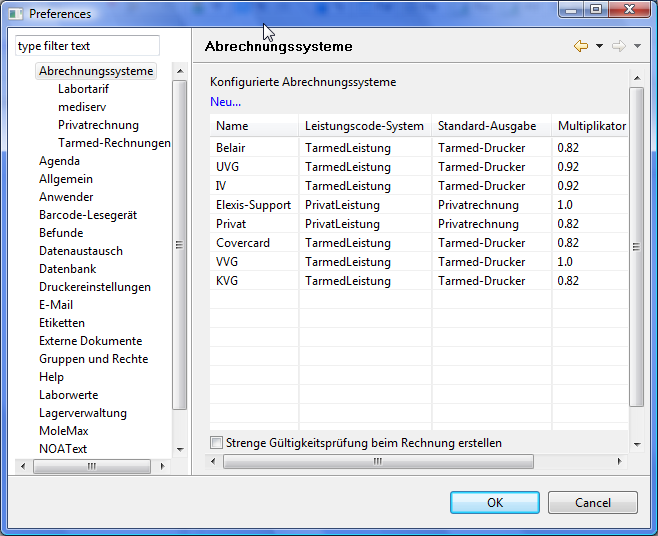
\includegraphics[width=0.9\textwidth]{abr1}\\
  \caption{Abrechnungssysteme: Übersicht}\label{fig:abr1}
\end{figure}
Es kann beliebig viele Abrechnungssysteme geben, und die Namen der einzelnen Abrechnungssysteme sind seitens Elexis egal. Um alle Schweizer Systeme abzudecken, sollten allerdings Abrechnungssysteme mit den Namen 'KVG', 'UVG', 'IV', 'MV' und 'VVG' vorhanden sein. Weitere können nach Belieben dazukommen. Es ist beispielsweise problemlos möglich, zwei verschiedene KVG-Systeme mit verschiedenen Taxpunktwerten zu definieren.

\medskip

Um ein neues Abrechnungssystem zu erstellen, klickt man auf 'Neu...', um ein bestehendes zu modifizieren, klickt man doppelt darauf. Es öffnet sich der Abrechnungssystem-Konfigurationsdialog (Abb. \ref{fig:abr2}.
\begin{figure}
  % Requires \usepackage{graphicx}
  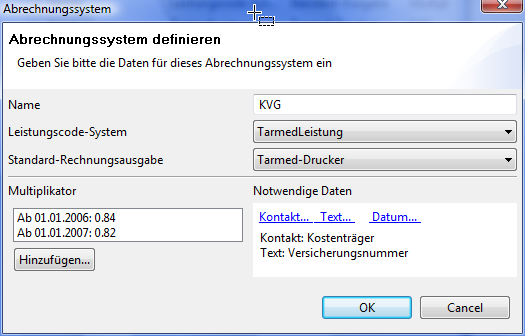
\includegraphics{abr2}\\
  \caption{KVG-Abrechnungssystem}\label{fig:abr2}
\end{figure}
Der Name ist wie gesagt frei wählbar. Für Leistungscode-System und Standard-Rechnungsausgabe können Sie aus den von den vorhandenen Abrechnungs-Plugins beigesteuerten Optionen wählen. Der Multiplikator ist die anzuwendende Tarifstufe (der 'Taxpunkt') für dieses System. Ein Multiplikator muss immer in Form einer Dezimalzahl angegeben werden und gilt immer ab einem bestimmten Datum so lange, bis ein anderer Multiplikator definiert wird. \textbf{Ein einmal eingegebener Multiplikator kann weder gelöscht noch geändert werden!}

Unter 'Notwendige Daten' geben Sie an, was für Angaben vorhanden sein müssen, damit ein Fall, der dieses Abrechnungssystem hat, als gültiog betrachtet wird. Solche Angaben können ein Kontakt sein, wie z.B. Kostenträger, oder ein Text, wie z.B. Versicherungs- oder Unfallnummer oder Vertragsnummer etc., oder es kann ein Datum sein, z.B. ein Unfalldatum.
Implizit immer notwendig ist der Kontakt 'Rechnungsempfänger', der deshalb hier nicht separat eingetragen werden darf.
Durch Rechtsklick kann man einen Eintrag in dieser Liste wieder löschen. Sie sehen das, was Sie hier eingegeben haben wieder unter den 'Fall-Details' als Fall-Erfordernisse (s. \ref{fall-erfordernisse}, S. \pageref{fall-erfordernisse}).

\subsection{Mandanten und Rechnungssteller}

Jeder Kontakt zwischen der Praxis und einem Patienten steht unter der Verantwortung eines \textit{Mandanten} und geht auf Rechnung eines \textit{Rechnungsstellers}. Im einfachsten und in der Schweiz üblichen Fall sind Mandant und Rechnungssteller identisch. Es ist aber auch möglich, dass ein Mandant im Fixlohn angestellt ist, auf eigen Verantwortung arbeitet, aber für einen anderen Rechnungssteller abrechnet (z.B. in einem HMO-Zentrum oder einer Polikinik). Dies ist nicht zu verwechseln mit einem Assistenten: Ein Assistent ist selber kein Mandant, sondern arbeitet auf Rechnung und unter der Verantwortung eines Mandanten.

\medskip

Einen Mandanten erstellt man, indem man ihn unter den \textit{Kontakten} anlegt und das Häkchen 'Mandant' ankreuzt. Danach kann man unter \textsc{Datei-Einstellungen-Mandanten} Benutzername und Passwort eingeben und festlegen, für welchen REchnungssteller dieser Mandant arbeitet.

Diese Zusammenhänge sind auch im Elexis-Handbuch beschrieben, genaueres bitte ich dort nachzulesen.

\medskip

Zurück zum Tarmed-System: Wenn das Plugin 'elexis-arzttarife-schweiz' installiert ist, finden Sie unter \textsc{Datei-Einstellungen-Abrechnungssysteme} auch die Positionen 'Labortarif' und 'Tarmed-Rechnungen' (S. Abb. \ref{fig:abr1}). Wählen Sie zunächst den Punkt Labortarife (Abb. \ref{fig:abr3}):
\begin{figure}
  % Requires \usepackage{graphicx}
  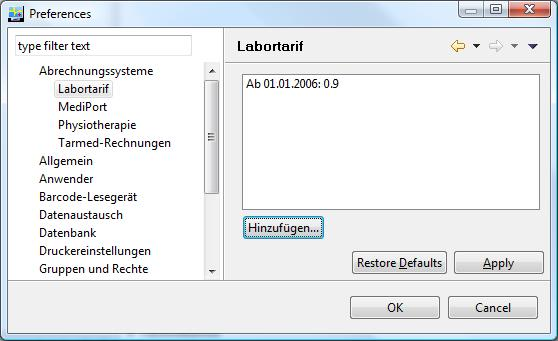
\includegraphics{abr3}\\
  \caption{Labor-Taxpunkt}\label{fig:abr3}
\end{figure}
Hier muss der Multiplikator gleich wie bei den Abrechnungssystemen eingegeben werden. Auch hier kann ein einmal eingetragener Wert nicht mehr geändert werden und er ist ab dem Stichdatum bis zur nächsten Änderung gültig.

\medskip

Gehen Sie dann zum Punkt 'Tarmed-Rechnungen'. Es erscheint ein Dialog wie in Abb.\ref{fig:abr4}.
\begin{figure}
    \center
  % Requires \usepackage{graphicx}
  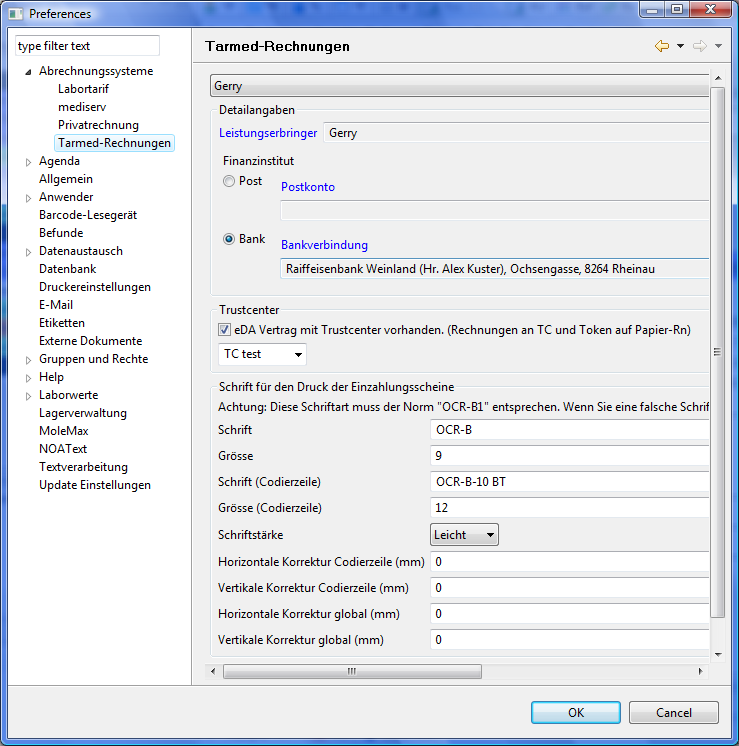
\includegraphics[width=0.85\textwidth]{abr4}\\
  \caption{Tarmedrechnungs-Einstellungen}\label{fig:abr4}
\end{figure}

Hier müssen Sie für jeden Mandanten und Rechnungssteller \textit{separat} alle für die Abrechnung relevanten Daten eingeben. Wählen Sie also im Combobox.Feld ganz oben zunächst einen Mandanten aus. Dadurch erscheint im Feld hinter 'Leistungserbringer' der Name dieses Mandanten. Klicken Sie dann auf das blaue Wort 'Leistungserbringer'. Es öffnet sich eine Dialogbox wie in Abb \ref{fig:abr5}.
\begin{figure}
  % Requires \usepackage{graphicx}
  \center
  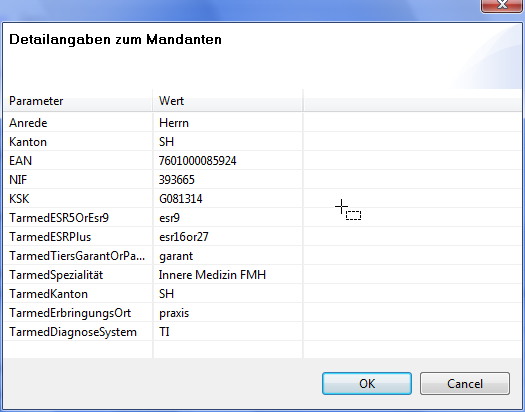
\includegraphics[width=0.75\textwidth]{abr5}\\
  \caption{Einstellung pro Mandant}\label{fig:abr5}
\end{figure}

Um eine Zeile zu ändern müssen Sie in dieser Zeile die \textbf{Eingabetaste} drücken, dann den neuen Wert eingeben, dann nochmal die \textbf{Eingabetaste} drücken und erst dann mit der Maus oder der Pfeiltaste ein anderes Feld aufsuchen.

Die Bedeutung der einzelnen Zeilen ist:
\begin{itemize}
\item Anrede: Sie haben es erraten ;-)
\item Kanton: Der Standort Ihrer Praxis. Wenn Sie in mehreren Kantonen praktizieren, müssen Sie einen eigenen Mandanten für jeden Kanton erstellen (z.B. Müller TI und Müller AG).
\item EAN: Ihre europäische Artikelnummer (Ja, wenn Sie ein in der Schweiz zugelassener Arzt sind, dann sind Sie auch ein europäischer Artikel, vergleichbar einer Milchtüte oder einem Badeschwamm). Falls Sie Ihre EAN nicht kennen, wenden Sie sich an die FMH.
\item NIF: Wenn Sie IV-Fälle behandeln, benötigen Sie eine Nummer der IV, die sich NIF nennt. Fragen Sie mich nicht, wieso die IV nicht die EAN verwenden kann.
\item KSK: Santésuisse hat Ihnen eine ZSR- oder KSK-Nummer gegeben, damit Sie über die Kassen abrechnen dürfen. Geben Sie diese Nummer ohne Punkte, Striche oder Leerzeichen ein. Und fragen Sie mich nicht, wieso Santésuisse nicht die EAN oder die NIF verwendet.
\item TarmedESR5OrEsr9: Das zu verwendende ESR-System. Fragen Sie  nicht, sondern schreiben Sie 'esr9'. Ausser, wenn Sie genau wissen, was Sie tun. Aber dann brauchen Sie eh nicht zu fragen.
\item TarmedEsrPlus: Dito. Schreiben Sie im Zweifelsfall einfach 'esr16or27'.
\item TarmedTiersGarantOrPayant: Schreiben Sie garant oder payant je nach Ihrem bevorzugten Abrechnungssystem. Hat aber zur Zeit nicht viel Konsequenz, was Sie da hinschreiben.
\item TarmedSpezialität: Der Titel, der Ihre 'Dignität' definiert. Fragen zum  Dignitätskonzept beantworten gerne und erschöpfend TarmedSuisse und die FMH.
\item TarmedKanton Nochmal der Praxisstandort.
\item TarmedErbringungsOrt praxis oder klinik (Wo Sie Ihre Leistungen erbringen)
\item TarmedDiagnoseSystem: Nach welcher Systematik Sie standardmässig Diagnosen auf den Rechnungen angeben. Schreiben Sie TI für Tessiner-Code, ausser wenn Sie einen guten und von TarmedSuisse abgesegneten Grund haben, etwas anderes zu schreiben.
\end{itemize}

Klicken Sie dann auf 'OK' um diesen Dialog wieder zu schliessen und wieder zu Abb.\ref{fig:abr4} zurückzukommen.


\subsection{Post- oder Bankkonto}
Jetzt müssen Sie das Konto angeben, auf das Sie die Zahlungen für Ihre Rechnungen erwarten. Sie benötigen ein VESR oder BESR Konto, zusammenfassend auch ESR-Konto genannt. Ein VESR-Konto ist ein ESR-Konto bei der Post, ein BESR-Konto ist eines bei einer Bank. Ein ESR-Konto ist eines, das mit diesen orangen (früher blauen) Einzahlungsscheinen befüllt wird, auf denen eine Referenznummer steht und deren Mitteilungskästchen mit einem vorgedruckten 'Keine Mitteilungen anbringen' beschriftet ist.

Das schöne an ESR-Konti ist, dass Dateien mit Zahlungseingängen automatisch eingelesen und verarbeitet werden können, so dass Sie die Zahlungen nicht manuell verbuchen müssen, sondern diese Aufgabe an den Computer delegieren können.

\medskip

 \textbf{Dringende Empfehlung} Falls Sie schon ein ESR-Konto haben, das Sie mit einem anderen Programm benutzen, eröffnen Sie ein neues für die Benutzung mit Elexis, weil sonst die ESR-Zeilen nicht bzw. falsch interpretiert werden und beide Programme bei jedem Einlesen Fehlermeldungen ausspucken werden!

\medskip

Eröffnen Sie also je nach Geschmack bei der Post oder Ihrer Lieblingsbank ein ESR-Konto. Klicken Sie je nachdem auf das blaue Wort 'Postkonto' oder 'Bankverbindung'\footnote{Im Fall von 'Bankverbindung' muss Ihre Bank zuvor als Kontakt erfasst worden sein}.

\begin{figure}[htbp]
     \begin{minipage}{0.5\textwidth}
      \centering
       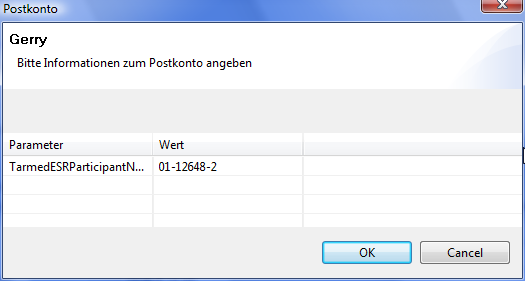
\includegraphics[width=0.95\textwidth]{abr6}
       \caption{VESR (Post)}
       	\label{fig:abr6}
     \end{minipage}\hfill
     \begin{minipage}{0.5\textwidth}
      \centering
       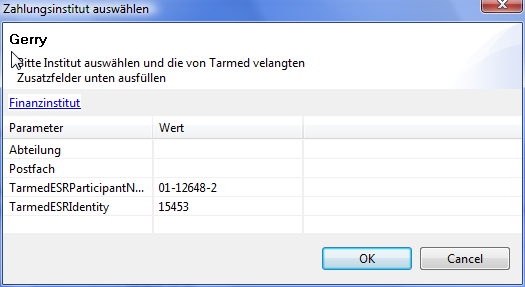
\includegraphics[width=0.95\textwidth]{abr7}
       \caption{BESR (Bank)}
       \label{fig:abr7}
     \end{minipage}
   \end{figure}

Je nach Auswahl erscheint eine Dialogbox wie Abb. \ref{fig:abr6} oder Abb. \ref{fig:abr7}. Beim Postkonto müssen Sie nur die VESR-Teilnehmernummer eintragen, die Sie von der Post erhalten haben. Beim Bankkonto benötigen Sie zunächst die Bank: Klicken Sie auf das blaue 'Finanzinstitut' und wählen Sie den hoffentlich zuvor angelegten Kontakt, der Ihre Bank beschreibt. Geben Sie dann neben TarmedESRParticipantNumber die VESR-Teilnehmernummer \textit{der Bank} ein. Neben TarmedESRIdentity müssen Sie die BESR-Identitätsnummer eingeben, die Sie von der Bank bekommen haben. Klicken Sie dann auf OK, um wieder zu Abb. \ref{fig:abr4} zurückzukommen.

\subsection{TrustCenter}
Da gibt es nicht viel zu sagen. Falls Sie einen TC-Vertrag haben, setzen Sie hier ein Häkchen und wählen Ihr TrustCenter aus. (Wenn Sie das tun, dann wird auf dem Rückforderungsbeleg von TG-Rechnungen ein passendes Token gedruckt, das beinahe wie eine ESR-Zeile aussieht, aber keine ist).

\subsection{Einzahlungsschein}
Elexis benötigt a4-Papier mit \textit{unten} integriertem ESR-Einzahlungsschein. Also das unterste Drittel der A4-Seite ist der orange Einzahlungsschein des Typs BESR oder VESR (bei ersterem steht eine Zeile 'zugunsten von' im Empfänger-Feld).

Zunächst benötigen Sie eine Schriftart des Typs OCR-B. diese Schriftart muss auf dem Computer installiert sein, von dem aus die Rechnungen gedruckt werden sollen \footnote{Tatsächlich empfehlen wir ausdrücklich, Rechnungen immer vom selben PC auf denselben Drucker auszugeben. Erst wenn das reibungslos funktioniert, können Experimente mit unterschiedlichen PC's gemacht werden, wenn es unbedingt sein muss.}. Nein, diese Schriftart ist nicht Bestandteil von Elexis, da sie lizenzpflichtig ist. Möglicherweise haben Sie aber von einem anderen ESR-fähigen Programm eine solche Schriftart irgendwo installiert und können diese verwenden. Ansonsten können Sie sich auch an die Post oder Ihre Bank wenden um zu erfahren, wo Sie diese Schriftart kaufen können.


Weil unterschiedliche Drucker das Papier nicht hunterprozentig identisch positionieren, und weil die Post ein wenig kritisch bezüglich der
Position der ESR-Zeile ist, kann man ausserdem den Ausdruck hier entsprechend konfigurieren. Sie benötigen ev eine ESR-Schablone, auf der Sie die korrekte Grösse und Positionierung der Codierzeile ablesen können.

Nun zu den Einstellungen:
\begin{itemize}
\item Unter 'Schrift' geben Sie diejenige Schriftart ein, die der Einzahlungsschein ausserhalb der ESR-Zeile haben soll. Nehmen Sie hier irgendetwas nach Ihrem Geschmack (es muss natürlich eine auf dem PC installierte Schriftart sein).
\item Unter 'Grösse' geben Sie die gewünschte Schriftgrösse in Punkt ein.
\item Unter 'Schrift (Codierzeile)' müssen Sie die OCR-B Schriftart angeben.
\item Mit 'Grösse (Codierzeile)' und der 'Schriftstärke' müssen Sie etwas experimentieren, bis Sie die korrekte OCR-lesbare Zeile haben
\item Horizontale Korrektur der Codierzeile: Mit positiven Werten schieben Sie die Codierzeile nach rechts, mit negativen nach links.
\item Vertikale Korrektur der Codierzeile: Mit positiven Werten schieben Sie die Zeile nach unten, mit negativen nach oben.
\item Horizontale Korrektur global: Wenn besipielsweise die Zahlen nicht schön in die Felder kommen, können Sie hier den Einzahlungsschein als ganzes verschieben. (Sie müssen danach allerdings vermutlich die Codierzeile wieder neu positionieren).
\item vertikale Korrektur global: Den ganzen Einzahlungsschein-Inhalt nach oben oder unten verschieben.
\end{itemize}

Dann können Sie diese Dialogbox schliessen.

\subsection{Druckvorlagen}
Wie (fast) alles, was in Elexis ausgedruckt wird, basieren auch Rechnungen auf Druckvorlagen. Bei Tarmed heissen diese System-Vorlagen:

\medskip

\begin{tabular}{|l|l|}
\hline
Tarmedrechung\_EZ & Tarmedrechnung mit ESR\\
Tarmedrechnung\_M1 & Erste Mahnung mit ESR\\
Tarmedrechnung\_M2 & Zweite Mahnung mit ESR\\
Tarmedrechnung\_M3 & Dritte Mahnung mit ESR\\
\hline
Tarmedrechnung\_S1 & Rückforderungsbeleg/TP-Rechnung erste Seite\\
Tarmedrechnung\_S2 & Rückforderungsbeleg/TP-Rechnung Folgeseite\\
\hline

\end{tabular}

\medskip

Diese Vorlagen sollten mit der Installation bereits vorhanden sein. Sie können die oberen 4 anpassen, aber es dürfen nur die oberen zwei Drittel des Blattes verwendet werden (das unterste Drittel wird der Einzahlungsschein). Achtung: Wenn Sie mehrere Mandanten haben und mandantenspezifische Texte verwenden, dann müssen Sie jede Vorlage mehrmals, einmal für jeden Mandanten, speichern. (Standardmässig sind die Rechnungsvorlagen für 'alle' gespeichert)

Die Seiten S1 und S2 sollten wenn überhaupt nur sehr vorsichtig geändert werden, da das Layout nicht geändert werden darf. Andernfalls sind es keine gültigen Tarmed-Rechnungen mehr.

Wie immer müssen Sie, wenn Sie eine Systemvorlage geändert haben, diese anschliessend explizit mit 'als Vorlage speichern... Systemvorlage' zurückspeichern, sonst gehen die Änderungen verloren.

\subsubsection{Druckvorlagen auf Drucker konfigurieren}
Sie müssen Elexis mitteilen, auf welchem Drucker und in welchem Schacht die Seiten mit ESR-Papier und die weissen Seiten ausgedruckt werden sollen. Beim NOAText-Plugin (Das ist das Textsystem, welches standardmässig unter Windows installiert ist), erfolgt diese Einstellung \textit{nicht} wie vielleicht erwartet unter \textsc{Datei-Einstellungen-Drucker}, sondern bei der Druckvorlage. Die Optionen unter \textsc{Datei-Einstellungen-Drucker} betreffend A4-Papier und ESR-Papier müssen in diesem Fall vielmehr sogar leer gelassen werden, damit die Druckkonfiguration gelingt!

\medskip

Um das Druckziel einzustellen, gehem Sie so vor: Laden Sie die betreffende Systemvorlage, z.B. 'Tarmedrechnung\_EZ' mit dem Menüpunkt \textsc{Systemvorlage laden} im lokalen Menu der Briefe-View. Wählen Sie dann im OpenOffice-Menu dieses Dokuments \textsc{Datei-Drucken...}. Geben Sie im Druckdialog unter 'Eigenschaften' den richtigen Drucker und Schacht ein.  Drucken Sie sie dann aus und schauen Sie, ob sie wirklich aus dem erwarteten Drucker und Schacht gedruckt wird. \textbf{Speichern} Sie dann die Vorlage wieder als Systemvorlage, und zwar unter demselben Namen, den sie vorher hatte. Wiederholen Sie diese Schritte für alle oben genannten Tarmedrechnungs-Vorlagen. (Dabei müssen \_S1 und \_S2 natürlich auf dem Schacht für weisses Papier ausgegeben werden, die anderen aus dem Schacht für ESR-Papier).

\section{Schritt für Schritt: Verrechnen, Rechnungen erstellen und ausgeben}
\label{rechnungenerstellen}
\subsection{Fälle, Rechnungsempfänger und Kostenträger}
Ein 'Fall' ist die Zuordnung eines Patienten zu einem Kostenträger und einer Identifikation des Kostenträgers für den Fall. Beispiel: Patient, Krankenkasse und Versicherungsnummer für KVG-Behandlungen oder Patient, Versicherung und Unfallnummer für UVG-Behandlungen, oder Patient, IV-Stelle und AHV-Nummer für IV-Behandlungen.

\medskip

Damit bleibt ein Fall auch immer so lange gültig, wie die Behandlungen demselben Versicherungsereignis zugeordnet bleiben. Ein KVG-Fall also bis der Patient die Kasse wechselt, ein UVG-Fall bis der Unfall abgeschlossen ist. Das Erstellen von Rechnungen hängt zunächst nicht damit zusammen -- Ein und derselbe Fall kann keine, eine oder mehrere Rechnungen haben. Es werden immer automatisch alle noch nicht verrechneten Konsultationen auf die nächste Rechnung genommen. (Ausser, wenn man es manuell anders macht).

\medskip

\textbf{Wichtig:} Ein einmal erstellter Fall ist wie ein Krankenkassenkärtli oder ein Unfallschein zu betrachten. Das heisst, er darf nicht mehr geändert werden. Wenn sich etwas an der Versicherung ändert, muss ein neuer Fall erstellt werden.

\subsubsection{Fall-Eigenschaften}
\label{fall-erfordernisse}
\begin{figure}
  % Requires \usepackage{graphicx}
  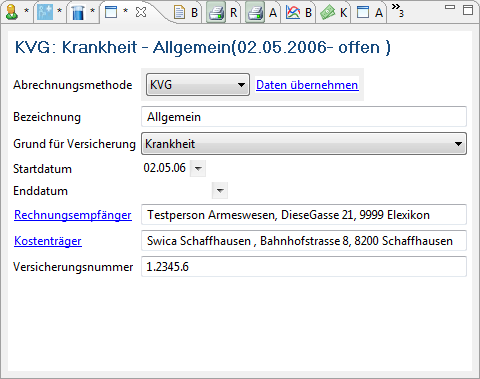
\includegraphics[width=0.7\textwidth]{abr8}\\
  \caption{Fall-Detail}\label{fig:abr8}
\end{figure}

Ein Fall ist immer einem Abrechnungssystem zugeordnet. Beim Erstellen eines neuen Falls muss im obersten Feld die 'Abrechnungsmethode' angegeben werden (s. Abb.\ref{fig:abr8}).
Darunter geben Sie eine Bezeichnung ein. Diese ist nur zur internen Markierung des Falles gedacht, damit Sie wissen, welcher Fall gemeint ist. Sie können hier irgendetwas schreiben, z.B. 'Beinbruch'.
Darunter das Feld 'Grund für die Versicherung' ist ein Tarmed-Erfordernis und wird auf der Rechnung erscheinen.
\textit{Startdatum} ist bei Unfällen idR das Unfalldatum, bei KVG-Behandlungen die erste Konsultation.
\textit{Enddatum} ist nur anzugeben, wenn der Fall abgeschlossen wird, also z.B. der Unfall abgeschlossen ist oder die Kasse gewechselt wird. Sobald ein Enddatum angegeben sit, ist der Fall als 'geschlossen' markiert und kann keine weiteren Konsultationen mehr aufnehmen.
Die nächsten Zeilen betreffen die für die Rechnungsstellung erforderlichen Daten. Diese hängen davon ab, was beim Erstellen des Abrechnungssystems dieses Falles definiert wurde.
Immer erforderlich ist der \textit{Rechnungsempfänger} - Wenn es keinen Rechnungsempfänger gibt, kann Elexis keine Rechnung erstellen.
Alle anderen Angaben hängen wie gesagt vom Abrechnungssystem ab.

Elexis betrachtet einen Fall als ungültig, wenn nicht alle Erfordernisse angegeben sind. Der Fall ist dann mit einem roten Punkt markiert. Wenn alle Erfordernisse eingetragen sind, wird der Punkt grün.

\subsubsection{Tiers Garant und Tiers Payant}
Tiers Payant bedeutet: Rechnungsempfänger und Kostenträger sind identisch. Tiers Garant bedeutet: Der Rechnungsempfänger ist nicht identisch mit dem Kostenträger. Es kann der Patient selbst sein, oder dessen Vormund, oder das Sozialamt. Tiers Soldant ist wiederum eine Variante von Tiers Payant, bei der der Kostenträger den nicht dem Selbstbehalt unterworfenen Anteil der Rechnung direkt an den Leistungserbringer zahlt.

Sie legen also beim Erstellen eines Falles fest, ob eine TP-Rechnung oder eine TG-Rechnung mit Rückforderungsbeleg erstellt wird: Wenn Sie für Kostenträger und Rechnungsempfänger denselben Kontakt auswählen, wird es TP, sonst TG.

\subsection{Rechnungen erstellen}
Es gibt zwei prinzipiell gleichwertige Möglichkeiten, Rechnungen zu erstellen: Sofortrechnung und (halb-)automatischer Rechnungslauf.

\subsubsection{Sofortrechnung}
Klicken Sie mit der rechten Maustaste in der 'Fälle'-View auf den Fall und wählen Sie 'Rechnung erstellen'. Es wird direkt eine Rechnung über alle noch offenen Konsultationen des aktuellen Mandanten des gewählten Falles erstellt.

\subsubsection{(halb-)automatischer Rechnungslauf}
Gehen Sie in die Rechnungen-Perspektive und öffnen Sie die View 'Konsultationen zum Verrechnen'. Hier findet sich in der linken Hälfte eine Liste aller noch unverrechneter Konsultationen des aktuellen Mandanten, gruppiert nach Patienten und Fällen. In der rechten Hälfte findet sich eine Liste derjenigen Konsultationen, die zum Rechnungserstellen vorgemerkt sind. Es gibt nun verschiedene Möglichkeiten, Konsultationen zwischen der linken und der rechten Liste zu verschieben:
\begin{itemize}
\item Alle Konsultationen aller Fälle eines Patienten: Ziehen Sie mit der Maus einen Patienteneintrag von der linken in die rechte Hälfte. Wenn Sie mehrere Patienten gleichzeitig auswählen wollen, können Sie wie in Windows gewohnt mit Druck auf die Shift- oder Ctrl-Taste und Mausklick mehrere auswählen und dann gemeinsam nach rechts ziehen. (Um \textit{alle} auszuwählen klicken Sie zunächst auf den ersten, dann mit 'Shift' auf den letzten Eintrag der Liste).
\item Alle Konsultationen eines Falles eines Patienten: Klicken Sie auf das (+)-Zeichen neben dem Patientennamen. Sie sehen alle Fälle, die noch unverrechnete Konsultationen enthalten. Ziehen Sie den gewünschten Fall in die rechte Hälfte.
\item Einzelne Konsultationen: Klicken Sie auf das (+)-Zeichen neben dem Fall. Sie sehen alle noch unverrechneten Konsultationen dieses Falles. Ziehen Sie eine oder mehrere ins rechte Feld.
\item Alle Konsultationen, die innerhalb eines bestimmten Zeitraums liegen: Öffnen Sie das View-Menu und wählen Sie 'Nach Datum auswählen'. Geben Sie in der dann öffnenden Dialogbox (Abb.\ref{fig:abr10}) das gewünschte Anfangs- und Enddatum ein.
\begin{figure}
  % Requires \usepackage{graphicx}
  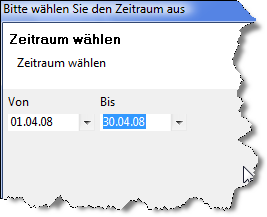
\includegraphics{abr10}\\
  \caption{Konsultationen nach Datum auswählen}\label{fig:abr10}
\end{figure}
    
\item Automatische Auswahl anhand verschiedener Kriterien: Klicken Sie das 'Zauberstab-Icon' und wählen Sie aus der Dialogbox wie Abb.\ref{fig:abr9} die gewünschten Kriterien aus:
\begin{figure}
  % Requires \usepackage{graphicx}
  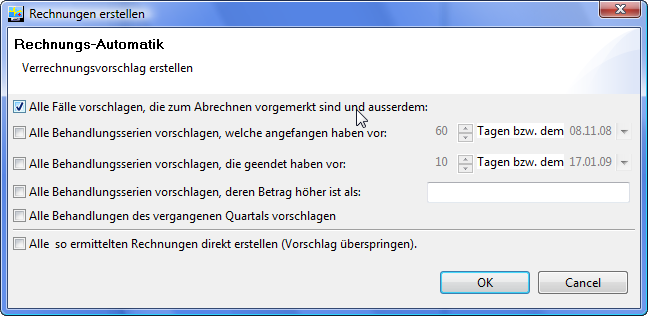
\includegraphics{abr9}\\
  \caption{Konsultationen automatisch auswählen}\label{fig:abr9}
\end{figure}
\begin{itemize}
    \item Alle Konsultationen einer Serie, deren erste vor einem bestimmten Datum war
    \item Alle Konsultationen einer Serie, deren letzte vor einem bestimmten Datum war
    \item Alle Konsultationen des vergangenen Kalenderquartals
    \item Alle Konsultationen, deren summierter Betrag eine bestimmte Höhe überschreitet.
    \end{itemize}
\end{itemize}

Je nach Gewohnheiten Ihrer Praxis werden Sie vermutlich nicht alle diese Methoden anwenden. In jedem Fall haben Sie anschliessend eine Anzahl Patienteneinträge in der rechten Hälfte des Fensters. Bis zu diesem Zeitpunkt ist noch nichts 'irreversibles' passiert. Sie können einzelne Einträge wieder entfernen, indem sie sie mit der rechten Maustaste anklicken und 'aus Auswahl entfernen' wählen. Sie können auch die ganze Auswahl wieder leeren, indem Sie auf das rote X - Symbol klicken. Oder Sie können die Auswahl ausdrucken, indem Sie auf das Druckersymbol klicken.

\medskip

Wenn Sie sicher sind, dass alles stimmt, können Sie nun aus der Auswahl Rechnungen erstellen lassen. \textbf{Achtung:} Dieser Schritt ist nicht mehr reversibel. Einmal erstellte Rechnungen können nicht mehr 'ungeschehen' gemacht werden. Klicken Sie also auf den Button 'Rechnungen erstellen'. 



\subsection{Rechnungen ausgeben}

\subsubsection{Ausgabeziele}

\subsubsection{Ausgabe auf Drucker}

\subsubsection{Ausgabe in XML-Datei}

\subsubsection{Ausgabe an Intermediär}

\section{Zahlungen verbuchen}

\subsection{Zahlungen manuell verbuchen}

\subsection{ESR-Files einlesen}
Die Post oder Ihre Bank teilt Ihnen eine Methode mit, wie Sie die Dateien mit den Zahlungseingängen (ESR-Dateien) erhalten können. Meist geht das heutzutage über dasselbe Internet-Portal, das Sie auch zum e-Banking verwenden. Manchmal werden die Files aber auch auf Diskette oder per verschlüsselter Mail geschickt.

\section{Mahnwesen}

\section{Merksätze}
\begin{itemize}
\item Eine Konsultation gehört immer zu genau einem Fall und genau einem Mandanten
\item Ein Fall gehört immer zu genau einem bestimmten Abrechnungssystem
\item Ein Fall ist unveränderlich wie ein Krankenkassenkärtli. Wenn etwas geändert werden muss, muss ein neuer Fall erstellt werden
\item Ein Fall kann Konsultationen mehrerer Mandanten beinhalten.
\item Eine Rechnung gehört immer zu genau einem Fall und genau einem Mandanten. Wenn ein Patient mehrere offene Fälle und/oder mehrere behandelnde Mandanten hat, wird für jeden Fall und jeden Mandanten eine separate Rechnung erstellt.
\item Eine einmal erstellte Rechnung ist unveränderlich. Sie kann nur storniert und neu erstellt werden.
\item Eingelesene ESR-Dateien müssen \textbf{sofort} verbucht werden, damit keine Zahlungseingänge verlorengehen.
\end{itemize}

\section{Weitere Unterstützung}
\subsection{Website}
Auf der Site http://www.elexis.ch werden aktuelle Informationen veröffentlicht. Es existiert auch eine Rubrik FAQ (Frequently Asked Questions), wo eventuell genau die Frage behandelt wird, die Sie auch grad stellen wollten. Schauen Sie also immer zuerst auf der Website nach. Diese enhält auch eine ausgezeichnete Suchfunktion, mit der Sie sowohl die ganze Site als auch nut die FAQ nach Stichwörtern durchsuchen können.

\subsection{Forum}
Unter http://www.elexis-forum.ch existiert ein Forum, in dem jede/r (auch Sie!) Fragen stellen und beantworten oder allgemeine Bemerkungen, Tips und Tricks, Kritiken usw. loswerden kann. Da Elexis ein community-Projekt sein will, wäre es schön, wenn Sie Fragen, die auf der Website nicht geklärt werden, im Forum besprechen würden, damit Andere auch etwas davon haben.
Wenn Sie sich als User im Forum angemeldet haben, dann können Sie es so einstellen, dass Ihnen automatisch nut die seit dem letzten Besuch neuen Themen angezeigt werden. Oder Sie können auch einen sog. RSS-Feed abonnieren, dann erhalten Sie jeweils die Titel der neuesten Beiträge als Newsfeed in Ihren Browser, ohne die Site aufsuchen zu müssen. Das Vorgehen, um Feeds zu abonnieren, ist in diesem Thread behandelt: http://www.elexis-forum.ch/viewtopic.php?t=10
Auch das Forum hat eine Suchfunktion, mit der Sie interessierende Themen nach Stichwörtern suchen können.

\subsection{Hilfe-Wiki}
Unter http://www.iatrix.org/pmwiki/pmwiki.php/Elexishilfe/Uebersicht existiert eine Hilfe-Seite, die ständig erweitert wird. Auch an dieser Seite können Sie aktiv mitmachen und eigene Erkenntnisse oder gelöste Probleme notieren, damit sie Anderen wieder zugute kommen.
Dieses Hilfe-Wiki wird standardmässig auch aufgerufen, wenn Sie von Elexis aus den 'Hilfe'-Button klicken, oder wenn Sie in irgendeiner View, zu der Sie Hilfe möchten, die F1-Taste drücken.


\end{document}
